\documentclass{article}
\usepackage{graphicx}
\usepackage{float}
\usepackage{geometry}
\geometry{a4paper, margin=1in}

\begin{document}

\section*{Øving 2: Databaser}

\subsection*{Oppgave 1: Relasjoner}
\subsubsection*{a) Forklaring av relasjoner}
\begin{itemize}
    \item 1:1 Relasjon:\\ Dette er når en rad i en tabell er relatert til nøyaktig én rad i en annen tabell
    \begin{itemize}
        \item Eksempel 1: En person har kun én pass-id, og pass-id er unikt for hver person.
        \item Eksempel 2: Et universitet har kun én offisiell rektor, og rektoren har kun ett universitetsid.
    \end{itemize}
    \item 1:n Relasjon: \\ Dette er når en rad i en tabell er relatert til flere rader i en annen tabell
    \begin{itemize}
        \item Eksempel 1: En lærer kan ha flere studenter, men en student har kun én lærer.
        \item Eksempel 2: En forfatter kan skrive flere bøker, men hver bok har kun én forfatter.
    \end{itemize}
    \item n:m Relasjon: \\ Dette er når flere rader i en tabell er relatert til flere rader i en annen tabell
    \begin{itemize}
        \item Eksempel 1: Studenter kan melde seg på flere kurs, og ett kurs kan ha flere studenter.
        \item Eksempel 2: Skuespillere kan medvirke i flere filmer, og en film kan ha flere skuespillere.
    \end{itemize}
\end{itemize}

\section*{Øving 2: Databaser}

\subsection*{Oppgave 2: Tabell "Auditorium"}
\subsubsection*{a) Normalformer}
\begin{itemize}
    \item 1NF: Tabellen oppfyller første normalform (1NF) siden hver celle inneholder bare en verdi, og hver kolonne er av samme datatype.
    \item 2NF: Tabellen bryter med andre normalform (2NF) fordi det er noen ikke-nøkkelattributter (HAdr og HTlf) som er avhengige av en delmengde av nøkkelen (HSkole), og ikke hele nøkkelen (AKodeID).
    \item 3NF: Tabellen bryter med tredje normalform (3NF) fordi det er transitive avhengigheter. HAdr og HTlf er avhengige av HSkole, som igjen er avhengig av AKodeID.
\end{itemize}

\subsubsection*{b) Lage tabeller}
\begin{itemize}
    \item Del opp tabellen Auditorium i to tabeller:
    \item \textbf{Auditorium:}
    \begin{itemize}
        \item AKodeID - Entydig kode for hvert enkelt auditorium (eks: AudMax, AudMin, AudG,…)
        \item AntPlass - Antall sitteplasser i auditoriet
        \item VKanon - Informasjon om hvorvidt auditoriet har videokanon installert
        \item PC - Informasjon om hvorvidt auditoriet har en pc installert
        \item HSkole - Informasjon om hvilken høgskole auditoriet tilhører (eks: HiA, …)
    \end{itemize}
    \item \textbf{Høgskole:}
    \begin{itemize}
        \item HSkole - Informasjon om hvilken høgskole auditoriet tilhører (eks: HiA, …)
        \item HAdr - Høgskolens adresse
        \item HTlf - Høgskolens telefonnummer (her ett telefonnummer pr høgskole)
    \end{itemize}
    \item Her er AKodeID og HSkole primærnøklene i Auditorium og Høgskole tabellene henholdsvis. Dette oppfyller 2NF og 3NF fordi det ikke er noen delvis eller transitive avhengigheter.
\end{itemize}
\begin{figure}[H]
    \centering
    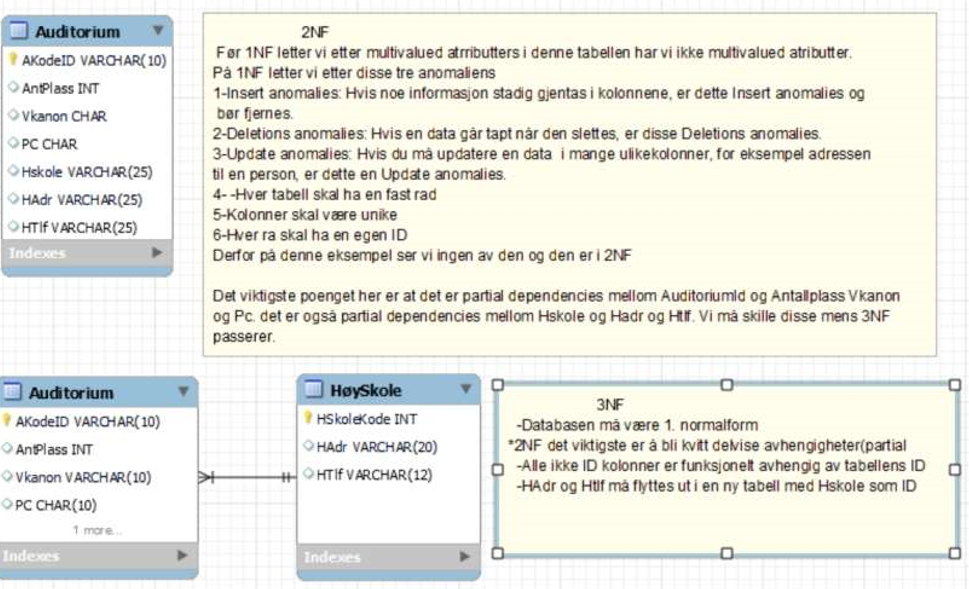
\includegraphics[width=0.6\textwidth]{2a&b.png}
    \caption{a og b}
    \label{fig:example}
\end{figure}

\subsubsection*{c) Splitt opp tabell for 3NF}
\begin{figure}[H]
    \centering
    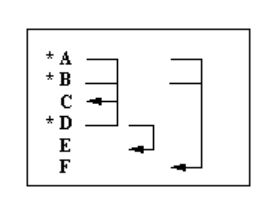
\includegraphics[width=0.6\textwidth]{oving2_c.png}
    \caption{fra oppgave}
    \label{fig:example}
\end{figure}
\begin{itemize}
    \item For å oppfylle tredje normalform (3NF), kan tabellen splittes opp i følgende måte:
    \item \textbf{Tabell 1:}
    \begin{itemize}
        \item Kolonner: A*, F
        \item Her er A primærnøkkelen.
    \end{itemize}
    \item \textbf{Tabell 2:}
    \begin{itemize}
        \item Kolonner: B*, C
        \item Her er B primærnøkkelen.
    \end{itemize}
    \item \textbf{Tabell 3:}
    \begin{itemize}
        \item Kolonner: D*, E
        \item Her er D primærnøkkelen.
    \end{itemize}
    \item \textbf{Tabell 4:}
    \begin{itemize}
        \item Kolonner: A*, B*, D*
        \item Her er A, B, og D primærnøklene.
    \end{itemize}
    \item I denne strukturen er det ingen transitive avhengigheter, og hver ikke-nøkkelattributt er fullstendig funksjonelt avhengig av hele nøkkelen. Derfor oppfyller denne strukturen tredje normalform (3NF).
\end{itemize}
\begin{figure}[H]
    \centering
    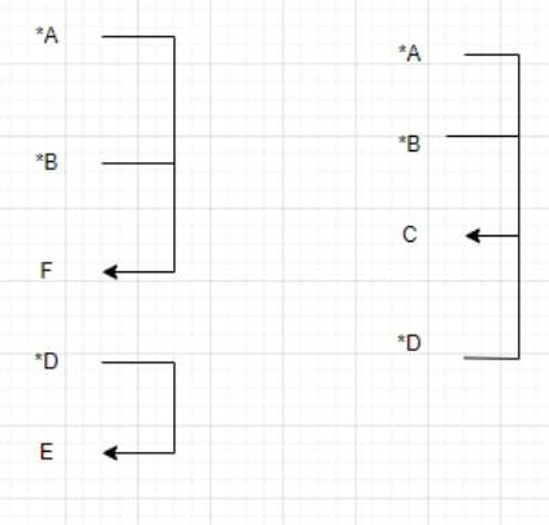
\includegraphics[width=0.6\textwidth]{2c.png}
    \caption{svar}
    \label{fig:example}
\end{figure}

\subsection*{Oppgave 3: Datamodell for legekonsultasjoner}
\subsubsection*{a) Datamodell}
\begin{figure}[H]
    \centering
    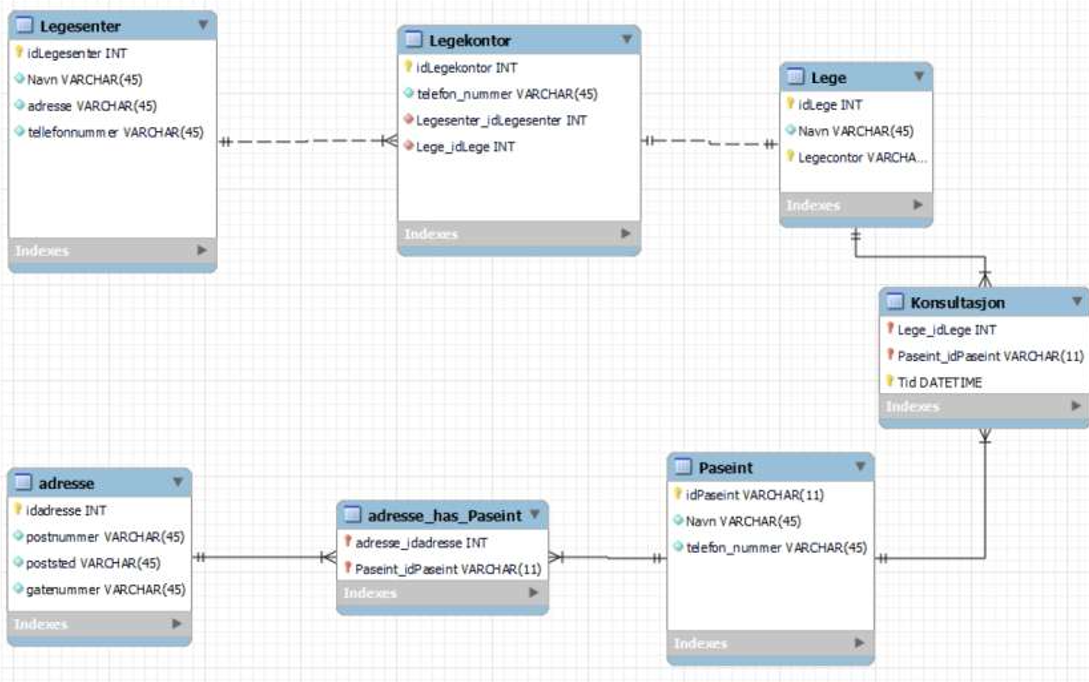
\includegraphics[width=0.6\textwidth]{3a&b.png}
    \caption{a og b}
    \label{fig:example}
\end{figure}
\begin{itemize}
    \item Legesenter (\underline{LegesenterNavn}, Adresse, Telefonnummer)
    \item Legekontor (\underline{KontorNummer}, Telefonnummer, \textit{LegesenterNavn})
    \item Lege (\underline{LegeKode}, Fornavn, Etternavn, \textit{KontorNummer})
    \item Pasient (\underline{Personnummer}, Fornavn, Etternavn, Adresse, Telefonnummer)
\end{itemize}

\subsubsection*{b) Forklaring av tabeller}
\begin{itemize}
    \item Legesenter (\underline{LegesenterNavn})
    \item Legekontor (\underline{KontorNummer}, \textit{LegesenterNavn})
    \item Lege (\underline{LegeKode}, \textit{KontorNummer})
    \item Pasient (\underline{Personnummer})
\end{itemize}

\subsection*{Oppgave 4: SQL-script}
\subsubsection*{a) MySQL-script for datamodellen i oppgave 3}
\begin{figure}[H]
    \centering
    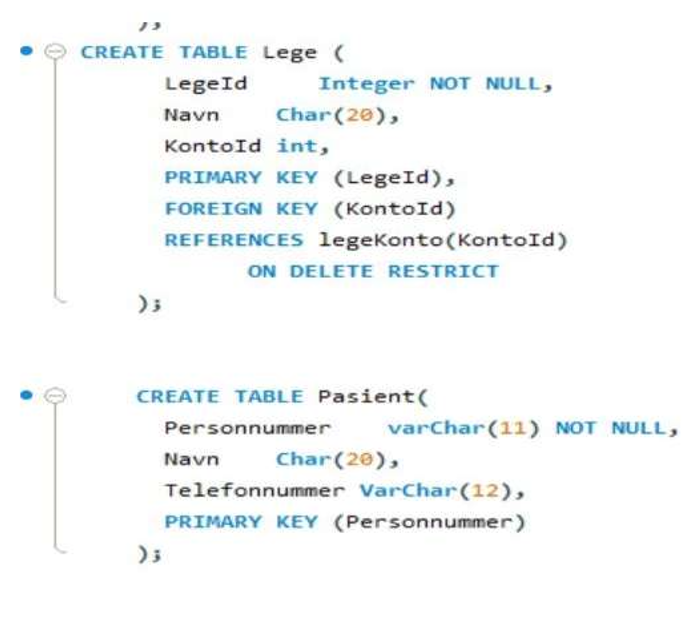
\includegraphics[width=0.6\textwidth]{4a2.png}
    \caption{svar}
    \label{fig:example}
\end{figure}
\begin{figure}[H]
    \centering
    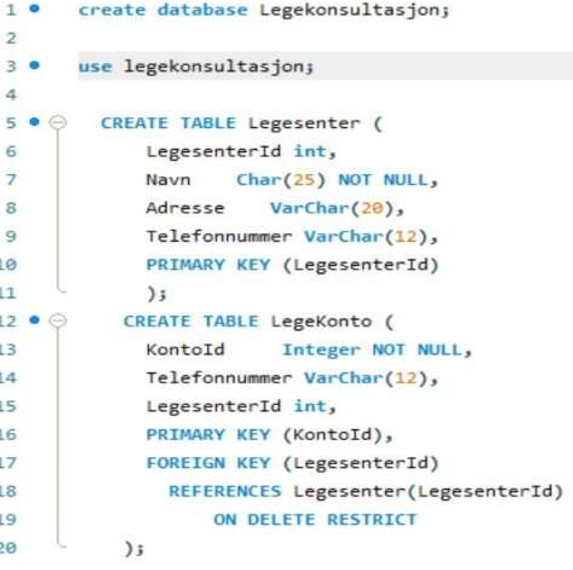
\includegraphics[width=0.6\textwidth]{4a1.png}
    \caption{svar}
    \label{fig:example}
\end{figure}

\subsubsection*{b) MySQL-script for å legge inn data}
\begin{figure}[H]
    \centering
    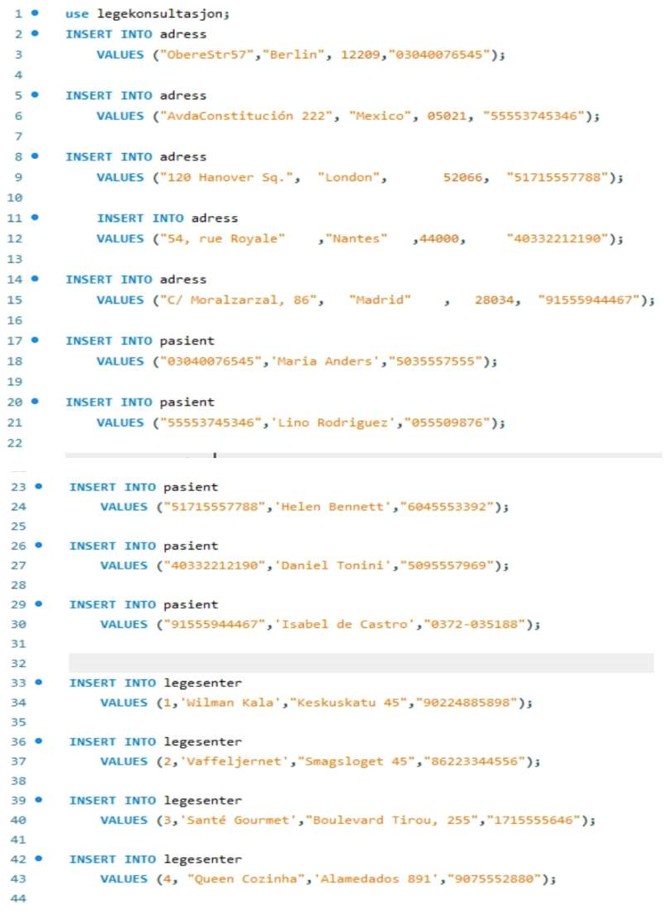
\includegraphics[width=0.6\textwidth]{4b.png}
    \caption{svar}
    \label{fig:example}
\end{figure}

\subsubsection*{c) Egendefinerte SELECT-spørringer}
\begin{figure}[H]
    \centering
    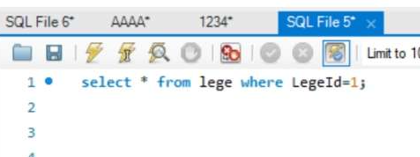
\includegraphics[width=0.6\textwidth]{4c1.png}
    \caption{spørring 1}
    \label{fig:example}
\end{figure}
\begin{figure}[H]
    \centering
    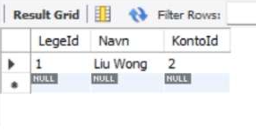
\includegraphics[width=0.6\textwidth]{4c2.png}
    \caption{spørring 1}
    \label{fig:example}
\end{figure}
\begin{figure}[H]
    \centering
    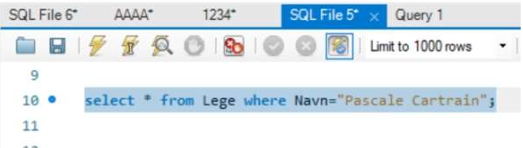
\includegraphics[width=0.6\textwidth]{4c3.png}
    \caption{spørring 2}
    \label{fig:example}
\end{figure}
\begin{figure}[H]
    \centering
    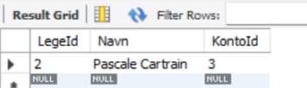
\includegraphics[width=0.6\textwidth]{4c4.png}
    \caption{spørring 2}
    \label{fig:example}
\end{figure}
\begin{figure}[H]
    \centering
    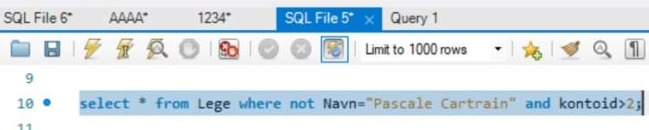
\includegraphics[width=0.6\textwidth]{4c5.png}
    \caption{spørring 3}
    \label{fig:example}
\end{figure}
\begin{figure}[H]
    \centering
    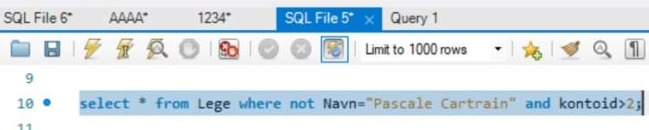
\includegraphics[width=0.6\textwidth]{4c5.png}
    \caption{spørring 3 }
    \label{fig:example}
\end{figure}
\end{document}
